\documentclass[letterpaper]{article} % DO NOT CHANGE THIS
\usepackage[submission]{aaai2027}  % DO NOT CHANGE THIS
% The serif, sans-serif, and monospaced fonts are loaded automatically by
% aaai2027.sty (newtxtext, helvet, courier). DO NOT add \usepackage{times},
% \usepackage{helvet}, \usepackage{courier}, or any other font package.
\usepackage[hyphens]{url}  % DO NOT CHANGE THIS
\usepackage{graphicx} % DO NOT CHANGE THIS
\urlstyle{rm} % DO NOT CHANGE THIS
\def\UrlFont{\rm}  % DO NOT CHANGE THIS
\usepackage{natbib}  % DO NOT CHANGE THIS AND DO NOT ADD ANY OPTIONS TO IT
\usepackage{caption} % DO NOT CHANGE THIS AND DO NOT ADD ANY OPTIONS TO IT
\frenchspacing  % DO NOT CHANGE THIS

% Algorithms (recommended by the AAAI author kit)
\usepackage{algorithm}
\usepackage{algorithmic}

% Recommended for better-looking tables
\usepackage{booktabs}

% Math
\usepackage{amsmath}
\usepackage{amssymb}
\usepackage{mathtools}

% Cross-references. Note: hyperref is forbidden by AAAI; cleveref without
% hyperref produces plain (non-linked) references, which is compliant.
\usepackage[capitalize,noabbrev]{cleveref}

% Keep the \pdfinfo as shown here.
\pdfinfo{
/TemplateVersion (2027.1)
}

% Section numbering is enabled (depth 2) because the paper cross-references
% numbered sections and subsections.
\setcounter{secnumdepth}{2}

\newcommand{\method}{SAGE}
\newcommand{\budget}{B}
\newcommand{\batchN}{N}

\title{SAGE: Self-Assessed Gradient-Based Enhancement for Test-Time Alignment of Large Language Models}
\author{
    Anonymous Submission
}
\affiliations{
}

\begin{document}
\maketitle

\begin{abstract}
We present \method{}, a test-time alignment method for refining large language model (LLM) outputs at inference time without retraining or relying on external reward models. \method{} uses the same LLM as both generator and self-judge: candidate responses are scored using a contrastive label judgment prompt and the resulting log-probability margin serves as a continuous preference signal. An iterative refinement algorithm then uses these scores to form good and bad candidate sets, extract a textual gradient, and guide subsequent hypothesis generations under a token budget. 
Across MATH-500, AlpacaEval, and XSTest, with Qwen3-8B and Llama-3.1-8B-Instruct, \method{} consistently improves accuracy and preference metrics relative to existing test-time alignment approaches, with ablations showing that these gains are robust under fixed inference budgets and do not rely on external reward models. The approach is resource-lean and plug-and-play, and we release the code and prompts to facilitate adoption.
\end{abstract}

\begin{links}
    \link{Code}{https://anonymous.4open.science/r/SAGE2026-8309}
\end{links}

\section{Introduction}


Large language models (LLMs) pre-trained on vast amounts of unlabeled text have demonstrated strong generalization across a wide range of downstream tasks. Nonetheless, real deployments often require adapting behavior to new domains, user preferences, or safety constraints without the time, data access, or compute needed for retraining. Test-time alignment addresses this need by improving outputs \textbf{during inference}, while keeping model weights fixed. It typically allocates a small amount of additional inference compute and elicits interpretable preference signals to steer generation toward more helpful responses aligned with user preferences \cite{litest}. This paradigm offers a practical path to domain adaptation and preference alignment under privacy, compliance, and latency constraints, without modifying the pretrained model.


Despite recent progress, existing state-of-the-art test-time alignment approaches, such as TPO \cite{litest} and ARGS \cite{khanov2024args}, still face several practical limitations. First, many of these methods rely on a separate reward model for scoring, which adds memory and latency overhead and introduces an additional component that can itself be misaligned or exploited. Second, relying solely on the single highest- and lowest-scoring responses for textual critiques can lead to noisy and outlier-sensitive feedback that fails to capture strengths or failure patterns across candidates, resulting in unstable or suboptimal refinement.


We propose \method{}, which treats the base LLM as both a generator and a soft self-judge. Instead of relying on an external reward model, \method{} elicits a contrastive log-probability label margin from a compact judging prompt, which enables fine-grained, model-internal preference scoring. A key component is an automatic contrastive grouping mechanism that forms representative good and bad sets, yielding a more stable textual `gradient' than extreme-only (best vs. worst) critiques and reducing sensitivity to outliers. The iterative loop then conditions generation on this gradient to refine future samples. In effect, \method{} leverages the LLM to surface its own implicit reward signal for test-time alignment, avoiding the need for additional reward models while operating under a small inference budget. An overview of \method{} in comparison to common test-time alignment variants is presented in \Cref{fig:taxonomy_compact}.


We conduct experiments on MATH-500 \citep{hendrycks2measuring}, AlpacaEval (including length-controlled LC win rate) \citep{dubois2024length}, and XSTest \citep{rottger2024xstest}, using Qwen3-8B \citep{yang2025qwen3} and Llama-3.1-8B-Instruct \citep{grattafiori2024llama}.\footnote{\textcolor{orange!85!black}{For Llama we use the W8A16 weight-quantized release (\texttt{Meta-Llama-3.1-8B-Instruct-quantized.w8a16}) to fit the serving budget; its absolute scores are accordingly lower than fp16 reference numbers.}} These benchmarks cover math reasoning (MATH-500), general instruction following (AlpacaEval), and safety/correctness stress tests (XSTest). We report accuracy on MATH-500/XSTest and win rate and length controlled (LC) win rate for AlpacaEval, comparing against commonly used inference-time baselines, including Best-of-\(N\), TPO \citep{litest} which relies on external reward model, and SPO \citep{xiang2025self}.
\method{} consistently improves performance across these benchmarks without relying on an external reward model. On Qwen3-8B, \method{} improves accuracy and preference metrics across all evaluated domains. AlpacaEval win rate vs. GPT-4 increases from 57.8 to 74.9, XSTest accuracy from 89.3 to 93.5, and MATH-500 accuracy from 84.4 to 92.0. \method{} also outperforms inference-time baselines that rely on explicit reward models (e.g., Best-of-\(N\)+RM, TPO) and generic LLM-as-a-judge approaches, under comparable budgets. The same procedure also applies to Llama-3.1-8B-Instruct, suggesting that \method{}’s self-judged textual-gradient refinement generalizes across model families.


We summarize our contributions as follows:
\begin{itemize}
    \item We introduce \method{}, a test-time alignment method in which the base LLM provides its own soft reward model via a contrastive label margin. As a result, the method avoids external reward models, reducing system complexity and potential reward signal misalignment.
    \item We design a grouped selection and textual-gradient mechanism that constructs good and bad sets and distills concise guidance from the judge. Compared to best–vs.–worst ranking-based feedback, this leads to more stable refinement by reducing sensitivity to outliers and improving transfer across iterations.
    \item We provide a practical self-judging recipe, called multi-aspect tagging with weights and confidence-threshold calibration, that turns discrete tags into a continuous score. This scoring scheme improves hypothesis ranking and provides a reliable correctness signal, particularly for verifiable tasks.
   
    \item Finally, we present an iterative test-time alignment procedure that integrates self-judged scoring, grouped selection, and textual gradients to progressively improve generations. Code, prompts, and scoring configurations are released to support reproducibility at: \url{https://anonymous.4open.science/r/SAGE2026-8309}.
\end{itemize}


    

    

    

    
    
    


\begin{figure}[t]
\centering
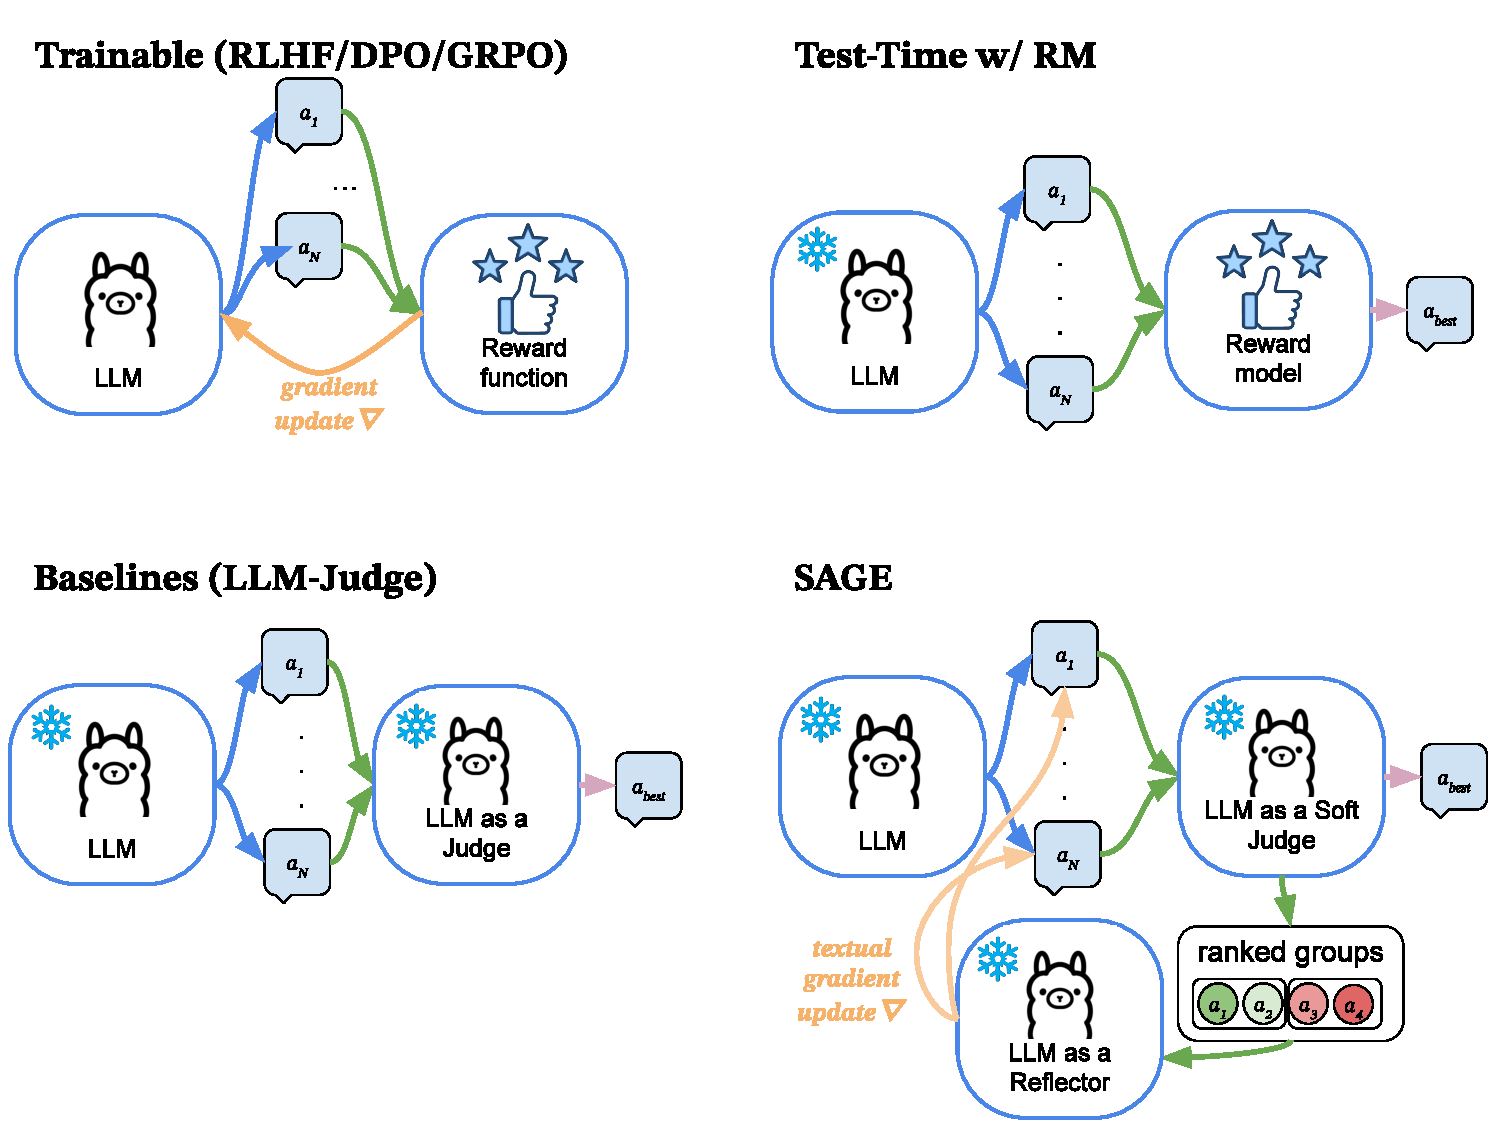
\includegraphics[width=\columnwidth]{figures/figure1_new_28012026.pdf}
\caption{Comparison between test-time alignment methods. \method{} acts post-training and uses the base LLM as generator, soft self-judge with a calibrated contrastive score, and textual-gradient extractor unlike LLM-as-judge heuristics or external RM–based scoring.}
\label{fig:taxonomy_compact}
\end{figure}


\section{Related Works}
\subsection{Preference alignment}
Aligning pretrained LLMs with human preferences is often approached by updating model parameters using preference supervision. Existing methods span point-wise optimization, such as policy-gradient variants like PPO \citep{schulman2017proximal}, ReMax \citep{li2024remax}, and KTO \citep{ethayarajh2024kto}, which adjust the model using scalar feedback on individual outputs, as well as pairwise optimization approaches that leverage relative judgments. A central strand is DPO \citep{rafailov2023direct}, which reformulates RLHF objectives to directly optimize the policy from pairwise comparisons. Subsequent work addresses overfitting and reduces reliance on reference policies, for example by constraining score gaps \citep{azar2023general}, or by removing or adapting the reference model \citep{meng2024simpo,kim2025sdpo,gorbatovski2024learn}. These training-time procedures are effective, but they require curated preference data and repeated fine-tuning, which can be slow to iterate and costly to deploy as requirements change.

\subsection{Test-time alignment}
Test-time alignment covers decoding heuristics, compute-allocation strategies, and judge-driven selection used at inference without changing model weights. Classical decoding includes greedy and beam search \citep{lowerre1976harpy}, which track multiple partial hypotheses. Although effective on structured tasks, these methods can over-concentrate probability mass and amplify local errors. Sampling-based decoding encourages diversity. For example, nucleus sampling \citep{holtzman2019curious} truncates low-mass tails, and contrastive search \citep{sucontrastive} penalizes degeneracy. However, both remain sensitive to hyperparameters.

Beyond fixed heuristics, adaptive search variants add flexibility, for example through alternative normalization schemes or affect-guided steering \citep{freitag2017beam,huang2023affective}, but they still rely on hand-tuned policies. A strong and widely used baseline is best-of-\(n\) (BoN): draw \(n\) candidates and pick the highest under a proxy. When paired with a reward model (RM), BoN+RM can deliver sizable gains via reranking \citep[e.g., human-feedback pipelines such as][]{stiennon2020learning}. However, it incurs additional RM training and maintenance costs and risks over-optimization when the proxy is misaligned. Replacing the RM with an LLM judge trades training for prompt engineering. In this setting, judge prompts can be used to verify intermediate steps (e.g., for math \citep{mahdavi2025scaling}) or elicit preferences. Test-time preference optimization frameworks \citep{litest} iterate textual feedback to improve candidates. These approaches often rely on discrete labels or scalarized heuristics, which can be coarse, sensitive to verbosity, and inefficient in their use of tokens.

Recent work scales test-time compute by allocating budget across perception, planning, and tool use \citep{zhu2025scaling} or by guiding sampling with intermediate checkpoints \citep{wang2025stepwise}, at the cost of controller complexity and extra hyperparameters. TreeBoN \citep{qiu2024treebon} speeds up BoN with speculative tree search driven by token-level preference signals.

Prompt-optimization methods aim to improve elicitation rather than search, for example through self-supervised prompt tuning \citep{xiang2025self}. However, these approaches often depend on seed exemplars and can struggle to transfer across domains.

\textcolor{green!50!black}{Same-model refinement is the setting closest to ours: Self-Refine \citep{madaan2023selfrefine} and Reflexion \citep{shinn2023reflexion} let one LLM draft, critique, and revise its own outputs through free-form feedback. A complementary line of work cautions how far self-evaluation can be trusted: models discriminate their own outputs no better than they generate them \citep{jiang2024selfincorrect}, judges favor familiar text \citep{wataoka2024selfpreference}, a shared generator-evaluator invites reward hacking \citep{pan2024spontaneous}, and verbalized confidence is imperfectly calibrated \citep{tian2023just}. We therefore score candidates contrastively against explicit rubrics and validate the selection signal against gold answers rather than assuming its reliability (\cref{sec:ablations}\textcolor{orange!85!black}{; judge--gold agreement and calibration are quantified in \cref{sec:app-judge-calibration}}); under a matched generation budget on MATH-500 this structured signal stays about two points ahead of free-form self-critique.}

In contrast, \method{} uses the base LLM as both generator and soft judge and replaces brittle discrete votes with a calibrated continuous margin computed directly from a judging prompt. The resulting score supports fine-grained ranking, and a concise textual “gradient” then steers subsequent sampling. This preserves BoN-style simplicity and avoids external reward models and heavy heuristics. The approach also fits strict token budgets through lightweight judging and caching.


    

    

    


\section{Proposed Method}
\label{sec:proposed-method}
\subsection{Notation and Problem setup}
\begin{figure*}[t]
\centering
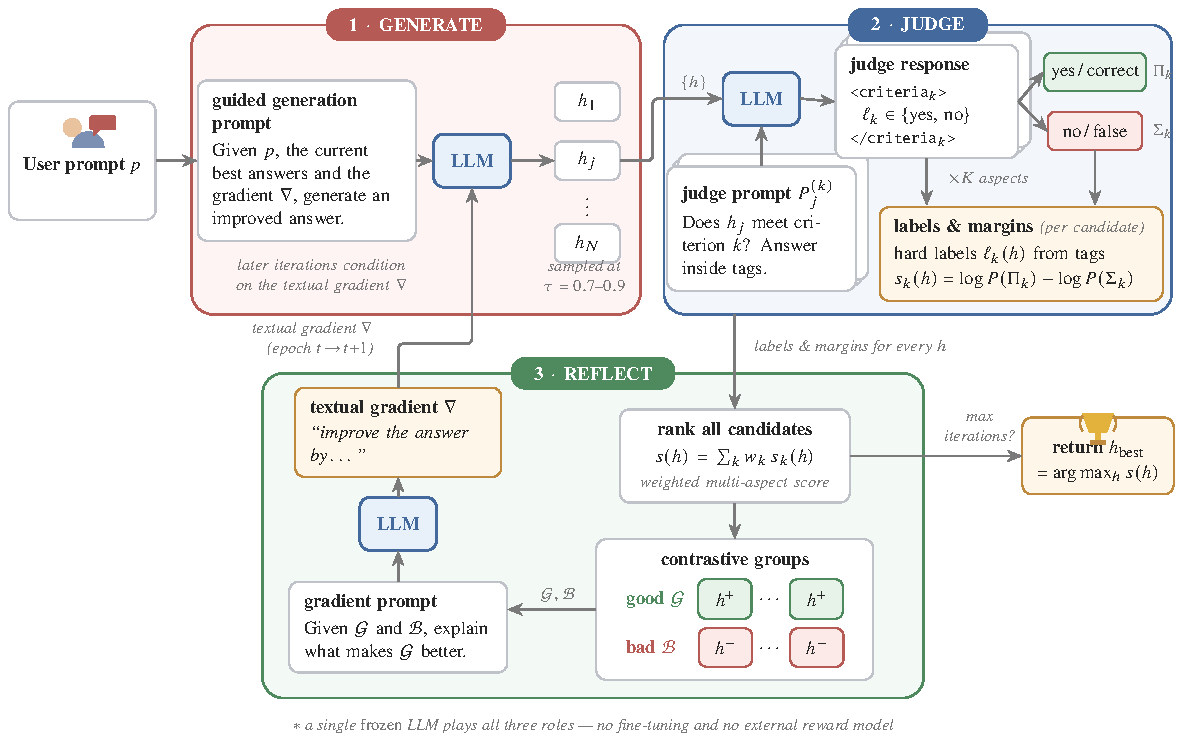
\includegraphics[width=\textwidth]{figures/sage_pipeline.pdf}
\caption{
  {The SAGE framework: a single LLM acts as generator, self-judge, and reflector. Candidates are scored with contrastive label margins, partitioned into good and bad groups, and a textual gradient $\nabla$ extracted from the groups guides the next generation round.}
}
\label{fig:sage_arch}
\end{figure*}


Let \(M\) denote a pretrained (frozen) language model. For a prompt \(p\in\mathcal{P}\), the model \(M\) induces a conditional policy \(\pi_{M}(h\mid p)\) over responses \(h\in\mathcal{X}\). At test time, alignment is typically driven by a scalar preference signal \(s(p,h)\), for example from a reward model or an LLM judge, which scores how well \(h\) matches human preferences. Our test-time alignment goal is to select a response that maximizes this signal, without updating \(M\):

\begin{equation}
h^\star(p)\;\in\;\arg\max_{h\in\mathcal{X}} s(p,h)\,,
\end{equation}

Concretely, test-time alignment methods implement a procedure that interacts with \(M\) to propose, score, and refine candidates at inference time.


We identify two practical shortcomings of existing test-time alignment approaches: First, many methods rely on a separate reward model for scoring, which adds memory, latency, and maintenance overhead and can introduce proxy mismatch or reward hacking. Second, forming a stable textual `gradient' for improving prior generations is difficult for methods that compare only the single best and worst candidates (e.g., TPO \cite{litest}): such extreme-only feedback is outlier-sensitive and often produces noisy guidance that fails to capture broader error patterns across the candidate set. In the next section, we describe our solution to address these limitations.


\subsection{SAGE}\label{method}
In this work, we propose \method{}, which uses a single LLM as the generator, the soft judge (reward model), and the textual-gradient estimator. The method assigns soft scores to rollouts and dynamically constructs contrastive groups to obtain a textual gradient, which is then used to further improve generation quality.

At a high level, \method{} uses the base LLM as both generator and soft judge. It draws small batches of candidates, scores them using a calibrated contrastive-label signal, aggregates evidence across groups to extract a concise textual `gradient', and conditions subsequent sampling on this guidance, all under a fixed token budget. An overview of the method is shown in \Cref{fig:sage_arch}.

\subsubsection{Initial generation}
At the beginning of the algorithm, we generate an initial set of rollouts (hypotheses) using the LLM as the generator and store them in the rollout set $\mathcal{H}$, which is updated in subsequent iterations. These rollouts are then scored by the judge.


\subsubsection{Judge}


\paragraph{Structured judge prompts and label sets.} We leverage the model’s \emph{implicit} preference signal at test time by asking the same LLM to judge its own outputs along a small set of human-interpretable aspects, such as usefulness, verification, completeness, and repetition. For each aspect \(k\in\{1,\dots,K\}\) we build a concise, deterministic judge prompt \(P^{(k)}_j(p,h)\) that specifies an aspect-specific rubric and includes the original task prompt \(p\) together with the candidate response \(h\in\mathcal{H}\), and requires the model to emit a decision inside dedicated tags, e.g. \texttt{<is\_useful>yes|no</is\_useful>} (see Appendix~\ref{sec:prompts-and-hyperparameters}). Parsing the tag yields a \emph{hard} label \(\hat\ell_k\in\Pi_k\cup\Sigma_k\), where \(\Pi_k\) (resp. \(\Sigma_k\)) is the set of positive (resp. negative) surface forms, e.g. \(\{\texttt{yes}\}\) and \(\{\texttt{no}\}\).

\paragraph{From tagged decisions to calibrated margins.} Beyond the hard tag, we use the model’s token-level probabilities to obtain \emph{soft} confidence score. Let \(u_k\) be the fixed prefix in \(P^{(k)}_j(p,h)\) up to, but not including, the first label token. For any \(\ell\in\Pi_k\cup\Sigma_k\), we estimate the conditional log-probability \(\log P(\ell\mid P^{(k)}_j,u_k)\) by summing the per-token log-probabilities for \(\ell\); if \(\ell\) is multi-token, we evaluate the full string using teacher forcing and aggregate over its canonical tokenizations via log-sum-exp.\footnote{With \(\Pi=\{\text{``yes''}\},\,\Sigma=\{\text{``no''}\}\), we aggregate over canonical variants of each word before forming the margin.} This yields a contrastive label margin for each aspect

  \begin{equation}
  \begin{aligned}
    s_k(h)\;=\;&\frac{1}{|\Pi_k|}\sum_{\ell\in\Pi_k}\log P\!\bigl(\ell\mid P^{(k)}_j,u_k\bigr)\\
    &-\;\frac{1}{|\Sigma_k|}\sum_{\sigma\in\Sigma_k}\log P\!\bigl(\sigma\mid P^{(k)}_j,u_k\bigr),
  \end{aligned}
  \end{equation}

which quantifies how strongly the judge prefers positive over negative outcomes for a given aspect.

\paragraph{Multi-aspect aggregation.} When multiple aspects are judged, we combine per-aspect margins with nonnegative weights \(w_k\) to form a scalar score

\begin{equation}
  s_{\mathbf{w}}(h)\;=\;\sum_{k=1}^{K} w_k\, s_k(h),
\end{equation}

used both to rank candidates and to form good and bad sets for the textual-gradient step. This construction makes the judge’s outputs \emph{explicit and auditable} via tags and it converts the model’s own confidence over labels into a \emph{calibrated} continuous preference signal for test-time alignment.

\paragraph{Calibration.} We apply a temperature separation using a lower temperature for judging than for generation to reduce variance. We find the margin is robust to minor prompt rewording, and that its monotonicity correlates with preference on math-style tasks. \textcolor{green!50!black}{Throughout, the margin serves as a ranking signal for selection and grouping; we do not rely on it as an absolute confidence estimate.}

\subsubsection{Reflection}
We form groups instead of comparing only extreme candidates. Contrasting a set of good responses \(\mathcal{G}\) with a set of bad responses \(\mathcal{B}\) yields a more stable and informative signal. By leveraging group-wise comparisons, we achieve more stable guidance and improved downstream transfer.
Group formation proceeds in three steps. Let \(\mathcal{H}\) denote the current pool of hypotheses and let \(\hat\ell_k(h)\in \Pi_k\cup\Sigma_k\) denote the \emph{hard} label emitted by the judge for aspect \(k\in\{1,\dots,K\}\) on candidate \(h\in\mathcal{H}\). With the aggregate margin \(s_{\mathbf w}(h)\) defined above, we construct \(\mathcal{G}\) and \(\mathcal{B}\) as follows (ties broken deterministically):
\begin{enumerate}
  \item \emph{Preliminary partition.} Define the preliminary good set
  \(\mathcal{G}_{\text{pre}}=\{\,h\in\mathcal{H}:\ \forall k,\ \hat\ell_k(h)\in \Pi_k\,\}\),
  i.e., candidates that are positive on all aspects; and the preliminary bad set
  \(\mathcal{B}_{\text{pre}}=\{\,h\in\mathcal{H}:\ \exists\,k\ \text{s.t.}\ \hat\ell_k(h)\in \Sigma_k\,\}\),
  i.e., candidates with at least one negative aspect.
  \item \emph{Within-set ranking and truncation.} Let \(m_{\min}\in\mathbb{N}\) be the per-group size cap: each side keeps at most \(m_{\min}\) candidates (fewer when the corresponding preliminary set is smaller). Rank \(\mathcal{G}_{\text{pre}}\) by decreasing \(s_{\mathbf w}\) and \(\mathcal{B}_{\text{pre}}\) by increasing \(s_{\mathbf w}\). Set
  \[
  \begin{aligned}
    \mathcal{G} &= \text{top }\min\!\bigl(|\mathcal{G}_{\text{pre}}|,\,m_{\min}\bigr)\ \text{of }\mathcal{G}_{\text{pre}},\\
    \mathcal{B} &= \text{bottom }\min\!\bigl(|\mathcal{B}_{\text{pre}}|,\,m_{\min}\bigr)\ \text{of }\mathcal{B}_{\text{pre}}.
  \end{aligned}
  \]
  \item \emph{Fallback when one side is empty.} If \(\mathcal{G}_{\text{pre}}=\varnothing\) (all candidates have at least one negative aspect), rank \(\mathcal{H}\) by \(s_{\mathbf w}\) and take
  \(\mathcal{G}=\) top \(m_{\min}\) of \(\mathcal{H}\), \(\mathcal{B}=\) bottom \(m_{\min}\) of \(\mathcal{H}\).
  Symmetrically, if \(\mathcal{B}_{\text{pre}}=\varnothing\), set \(\mathcal{B}=\) bottom \(m_{\min}\) of \(\mathcal{H}\) and \(\mathcal{G}=\) top \(m_{\min}\) of \(\mathcal{H}\).
\end{enumerate}
This procedure respects aspect-level hard decisions when available and uses the calibrated aggregate margin \(s_{\mathbf w}\) to prioritize stronger evidence within each side. When the hypothesis pool $|\mathcal{H}|$ is sufficiently large, it yields nonempty sets $\mathcal{G}$ and $\mathcal{B}$, which stabilizes the subsequent textual-gradient step.


Each iteration thus scores the pool with cached margins, partitions it into good and bad sets, asks the LLM to summarize the changes that would turn bad responses into good ones (the textual ``gradient''), and conditions the next \(\min(\batchN,\ \budget-\text{spent})\) samples on this guidance; we stop when \(\budget\) is exhausted or the epoch limit is reached and return the highest-scoring hypothesis (\cref{alg:method}).


\begin{figure}[t]
\centering
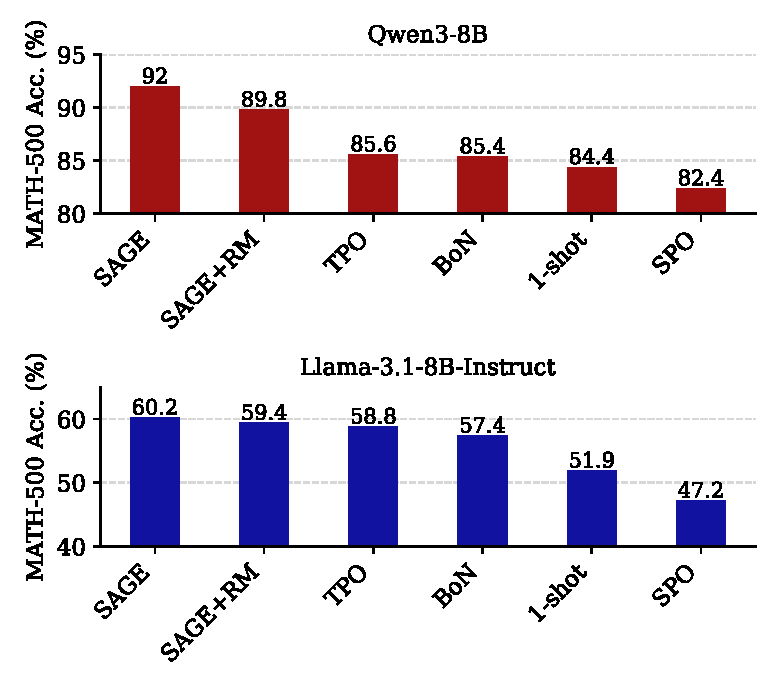
\includegraphics[width=0.86\columnwidth]{figures/headline_math500.pdf}
\caption{Results for \method{} on MATH-500 accuracy (\%). \method{} outperforms strong inference-time baselines across different model families. The internal self-judge consistently yields higher final scores than external reward models on math reasoning (\method{}+RM).}
\label{fig:headline_math_single}
\end{figure}

\subsubsection{Guided generation and scheduling}
The generation of subsequent hypotheses is conditioned on the original user prompt \(p\), a concise form of the gradient \(g\), and the \(k\) top-scoring exemplars from \(\mathcal{G}\) under the composite score \(s_{\mathbf{w}}(h)\). The decoding temperature is annealed over iterations, nucleus and top-\(k\) constraints are kept moderate, and maximum length is bounded to control judge cost. We also allow occasional ``exploration'' samples that ignore \(g\) with low probability to avoid premature convergence.

\begin{algorithm}[t]
\caption{\method{}: Self-judged iterative response refinement over \(T\) epochs}
\label{alg:method}
\begin{algorithmic}
   \STATE {\bfseries Inputs:} prompt \(p\); number of epochs \(T\); per-iteration batch size \(\batchN\); judge prompts \(\{P^{(k)}_j\}_{k=1}^K\); aspect weights \(\{w_k\}\); group-size cap \(m_{\min}\)
   \STATE {\bfseries Initialize:} hypothesis pool \(\mathcal{H} \leftarrow \{\}\); cache \(\mathcal{C}\leftarrow \{\}\)
   \STATE {\bfseries Step 0:} Sample \(\batchN\) hypotheses from \(M\) conditioned on \(p\); add to \(\mathcal{H}\)
   \FOR{\(t=1\) to \(T\)}
     \STATE For each \(h\in\mathcal{H}\): obtain hard labels \(\hat\ell_k(h)\in\{\Pi_k\cup\Sigma_k\}\) and per-aspect margins \(s_k(h)\); compute \(s_{\mathbf{w}}(h)=\sum_{k=1}^K w_k\, s_k(h)\); update \(\mathcal{C}\)
     \STATE Build preliminary sets \(\mathcal{G}_{\text{pre}}=\{h\in\mathcal{H}: \forall k,\, \hat\ell_k(h)\in \Pi_k\}\), \(\mathcal{B}_{\text{pre}}=\{h\in\mathcal{H}: \exists k,\, \hat\ell_k(h)\in \Sigma_k\}\)
     \STATE Rank \(\mathcal{G}_{\text{pre}}\) by decreasing \(s_{\mathbf{w}}\) and \(\mathcal{B}_{\text{pre}}\) by increasing \(s_{\mathbf{w}}\); set \(\mathcal{G}\leftarrow\) top \(\min(|\mathcal{G}_{\text{pre}}|,m_{\min})\), \(\mathcal{B}\leftarrow\) bottom \(\min(|\mathcal{B}_{\text{pre}}|,m_{\min})\); if a side is empty, take top/bottom \(m_{\min}\) from \(\mathcal{H}\) by \(s_{\mathbf{w}}\)
     \STATE Query textual gradient \(g \leftarrow \text{LLM\_improvements}(\mathcal{G}, \mathcal{B}, \{P^{\!(k)}_j\}, \{w_k\})\)
     \STATE Condition on \((p, g)\) and top exemplars from \(\mathcal{G}\); sample \(\batchN\) new hypotheses from \(M\); add them to \(\mathcal{H}\)
   \ENDFOR
   \STATE {\bfseries Return:} \(\arg\max_{h\in\mathcal{H}} s_{\mathbf{w}}(h)\)
\end{algorithmic}
\end{algorithm}

\section{Experiments}
\label{sec:experiments}
We evaluate \method{} with Qwen3-8B \citep{yang2025qwen3} and Llama-3.1-8B-Instruct \citep{grattafiori2024llama} on MATH-500, AlpacaEval and XSTest. We report task metrics and preference-based wins, and study sensitivity to temperatures, the number of optimization epochs and the sampling sizes.

\subsection{Benchmarks and setup}
We compare against state-of-the-art test-time methods, including Test-time Preference Optimization (TPO) and Self-supervised Preference Optimization (SPO), as well as simpler baselines such as Best-of-\(N\) sampling and zero-shot generation.

\subsection{Implementation details}
We use Qwen3-8B and Llama-3.1-8B-Instruct as the base models. For zero-shot generations, we use nucleus sampling with temperature of 0.7 and top-\(p\) set to 0.95.
For all evaluations that require a reward model, we use sfairXC/FsfairX-LLaMA3-RM-v0.1 \citep{dong2024rlhf}.

For SPO, we perform prompt tuning using GPT-4.1 as both the judge and the prompt editor. To ensure fair measurement, with no prompt calibration on evaluation items, we calibrate on five out-of-domain examples per task from a similar domain.
For MATH-500, we use AGIEval-Math \citep{zhongagieval}; for AlpacaEval we use a small subset of the Tulu instruction-following dataset \citep{lambert2024tulu}; and for XSTest we use Jailbreakbench \citep{chao2024jailbreakbench}. For TPO and Best-of-\(N\), we use the official TPO repository \citep{litest}. \textcolor{orange!85!black}{Because this calibration is deliberately minimal and out-of-domain (a single prompt tuned from five examples, with no access to evaluation items), SPO's win rates should be read as a compute-matched operating point rather than its unconstrained ceiling: SPO is designed to exploit a larger, in-domain prompt-optimization budget, which our inference-time-matched protocol does not grant it.}

By default, we use temperature of 0.7 for generation and 0.1 for judging. For math problems, we typically use a higher generation temperature in early stages to encourage solution diversity. We ablate both generation and judging temperatures on MATH-500, as reported in \cref{sec:ablations}. Prompts and evaluation criteria are provided in the Appendix.
For math-oriented tasks, we anneal the generation temperature from 0.8--1.0 in the initial stage to 0.7 in subsequent stages. Unless otherwise noted, we sample \(N=7\) hypotheses per generation stage and run two optimization epochs per benchmark, excluding the initial generation stage. Because the good and bad sets are selected automatically, we do not fix their sizes; the median size of each group is two to three hypotheses. \textcolor{orange!85!black}{Unless stated otherwise, results are single runs with a fixed seed; selected analyses are repeated over three seeds.} \textcolor{green!50!black}{Regarding cost, two optimization epochs with \(N=7\) average roughly 71 seconds per MATH-500 problem on one H200 GPU, against about 14 seconds for Best-of-\(N\) reranked by the same judge; the overhead is dominated by the extra hypothesis generations, as judging reads a few forced label tokens and margins are cached.} \textcolor{orange!85!black}{(H200 timings; the A100 wall-clock in \cref{tab:small-large-models} is correspondingly higher.)}


All Qwen3-8B experiments in \cref{tab:results-by-model} use the non-thinking mode to keep the evaluation setup uniform across experiments. Nevertheless, \method{} is equally applicable in reasoning mode: results on AIME~2026 \citep{dekoninck2026beyond} (Qwen3-8B and Qwen3.5-4B (thinking)), at additional model scales (Qwen3-1.7B, Qwen3-32B-FP8), and on further benchmarks (IFEval \citep{zhou2023instruction}, MMLU-Pro STEM \citep{wang2024mmlu}) \textcolor{blue}{are reported in \cref{sec:scaling-exp,sec:broader-benchmarks}}.

\subsection{Main results}
\noindent We report accuracy on MATH-500 and XSTest, and both pairwise win rate and length-controlled win rate on AlpacaEval.\footnote{\textcolor{orange!85!black}{AlpacaEval win rates are computed under a fixed in-house protocol (GPT-4 reference outputs, one judge configuration, all 805 instructions). Judge and reference versions differ from the live leaderboard, so absolute values are not comparable across papers; we rely on relative comparisons within each table.}} \Cref{tab:results-by-model} summarizes results for Qwen3-8B and Llama-3.1-8B-Instruct under \method{} alongside competitive baselines including TPO \citep{litest}, SPO \citep{xiang2025self}, Best-of-\(N\), and the base models.

For Qwen3-8B, \method{} performs best on both math and general tasks. On MATH-500, it reaches the accuracy of \(92.0\), outperforming the base model as well as both Best-of-\(N\) and TPO. On AlpacaEval, it attains a win rate of \(74.9\) and LC win rate of \(\textcolor{orange!85!black}{55.0}\), exceeding all baselines.  This advantage on math tasks appears to be driven by self-judging. Qwen3-8B evaluates the correctness of its own generations more reliably than an external reward model, which leads to steadier improvements and higher final scores (\cref{fig:judge-rm-dynamics,tab:rm-ablation}). \textcolor{green!50!black}{To rule out length effects, we ran a randomized head-to-head comparison of \method{} and base responses with a GPT-4.1 judge (200 prompts, response order randomized): \method{} is preferred in 57.5\% of pairs while its responses are marginally shorter at the median, so the gains reflect content rather than verbosity.}

Llama-3.1-8B-Instruct follows the same pattern. On MATH-500, it achieves an accuracy of \(60.2\), outperforming the base model as well as Best-of-N and TPO. It also shows clear gains on AlpacaEval with the win rate of \(49.2\) and LC win rate of \(47.1\), exceeding all baselines. On XSTest, \method{} is competitive or outperforms the baselines, achieving scores of \(93.5\) with Qwen and \(95.1\) with Llama. This indicates no trade-off between safety and correctness. \textcolor{green!50!black}{A per-category view of XSTest supports this: safe-prompt compliance improves by 3.6 points and unsafe-prompt refusal by 1.5, reducing exaggerated refusals without loosening guardrails.} Overall, \method{} consistently outperforms strong inference-time baselines without relying on an external reward model. The largest gains appear on math where self-judged correctness is particularly effective. \textcolor{blue}{Results for additional model scales (1.7B, 32B) and further benchmarks (AIME~2026, IFEval, MMLU-Pro STEM) follow in \cref{sec:scaling-exp,sec:broader-benchmarks}.}


\begin{table*}[t]
\centering
\begin{small}
\begin{sc}
\begin{tabular}{lcccc}
\toprule
\textbf{Variant / Model} & \textbf{MATH-500} & \textbf{AlpacaEval} & \textbf{AlpacaEval LC Winrate} & \textbf{XSTest} \\
\midrule
\multicolumn{5}{l}{\textbf{\method{}}} \\
Qwen3-8B & 92.0 & 74.9 & \textcolor{orange!85!black}{55.0} & 93.5 \\
Llama-3.1-8B-Instruct & 60.2 & 49.2 & 47.1 & 95.1 \\
\addlinespace
\multicolumn{5}{l}{\textbf{Baselines}} \\
Qwen3-8B (Base) & 84.4 & 57.8 & 50.1 & 89.3 \\
Qwen3-8B + Best-of-\(N\) & 85.4 & 68.8 & \textcolor{orange!85!black}{52.5} & 94.2 \\
Qwen3-8B + TPO & 85.6 & 72.4 & \textcolor{orange!85!black}{53.5} & 93.3 \\
Qwen3-8B + SPO & 82.4 & 9.7 & 17.6 & 90.2 \\
Llama-3.1-8B-Instruct (Base) & \textcolor{orange!85!black}{51.9} & 35.8 & 35.4 & 90.6 \\
Llama-3.1-8B-Instruct + Best-of-\(N\) & 57.4 & 44.7 & 43.05 & 94.4 \\
Llama-3.1-8B-Instruct + TPO & 58.8 & 48.01 & 41.39 & 93.3 \\
Llama-3.1-8B-Instruct + SPO & 47.2 & 7.7 & 12.8 & 91.1 \\
\bottomrule
\end{tabular}
\end{sc}
\end{small}
\caption{Results by model and benchmark. Metrics: MATH-500/XSTest = accuracy; AlpacaEval = win rate (\%)/LC-win rate. Top: \method{} (no external RM). Bottom: baselines including TPO \citep{litest}, SPO \citep{xiang2025self}, Best-of-\(N\), and Base; \method{}+RM variants are analyzed in \cref{tab:rm-ablation}.}
\label{tab:results-by-model}
\end{table*}

\subsection{Ablations}
\label{sec:ablations}
We compare \method{} using an external reward model against the same method using our internal judge. This comparison isolates the effect of the judging signal. As shown in \cref{tab:rm-ablation}, on Qwen3-8B the internal judge outperforms the external reward model variant, while on Llama-3.1-8B-Instruct the two perform comparably. This indicates that the calibrated internal signal provides a strong and lightweight alternative to reward model-based scoring.

\textcolor{orange!85!black}{A sharper test grades every candidate in the pool against the gold answer and asks whether the judge prefers incorrect but self-consistent responses. It does not: across three seeds on MATH-500, the margin separates correct from incorrect candidates (AUC 0.64) with no systematic preference for incorrect ones when a correct candidate is available; the self-judge tracks correctness rather than reinforcing the model's own mistakes.}

\textcolor{green!50!black}{Nor is the weakness of external reward signals on math an artifact of the particular reward model: Best-of-\(N\) selection with the recent Skywork-Reward-V2 model \citep{liu2025skywork} reaches only 74.2 on MATH-500 with Qwen3-8B, below the base model itself. A general-preference reward model misranks verifiable answers, and switching to a newer one does not remedy this.} \textcolor{orange!85!black}{External-RM reranking is thus inconsistent across reward models (cf. the one-point Best-of-\(N\) gain in \cref{tab:results-by-model}), while the self-judged margin requires no reward-model choice at all.}


\begin{table*}[t]
\centering
\begin{small}
\begin{sc}
\begin{tabular}{lcccc}
\toprule
\textbf{Variant / Model} & \textbf{MATH-500} & \textbf{AlpacaEval} & \textbf{AlpacaEval LC Winrate} & \textbf{XSTest} \\
\midrule
\method{} + RM (Qwen3-8B) & 89.8 & 74.7 & \textcolor{orange!85!black}{51.5} & 93.8 \\
\method{} + RM (Llama-3.1-8B-Instruct) & 59.4 & 48.3 & 47.5 & 95.1 \\
\method{} (Qwen3-8B) & 92.0 & 74.9 & \textcolor{orange!85!black}{55.0} & 93.5 \\
\method{} (Llama-3.1-8B-Instruct) & 60.2 & 49.2 & 47.1 & 95.1 \\
\bottomrule
\end{tabular}
\end{sc}
\end{small}
\caption{Ablation: \method{} with an external reward model (judging) vs. internal judge. Metrics as in \cref{tab:results-by-model}. \textcolor{orange!85!black}{For Llama on XSTest the RM tie-break never overrides the self-judge selection, hence identical scores; on AlpacaEval the RM-reranked variant selects longer responses at a similar raw win rate, which lowers its length-controlled score.}}
\label{tab:rm-ablation}
\end{table*}

\noindent We ablate the source of the scoring signal on MATH-500 using Qwen3-8B. Replacing an external reward model with our LLM-as-judge scoring improves performance under the same token budget and decoding settings. This result indicates that the contrastive-label margin derived from the base model provides a strong, low-overhead proxy for preference quality (see \cref{fig:ablation-qwen-math500}).

\noindent Judge-score dynamics across optimization epochs show a steady increase in the model’s self-judgment confidence on MATH-500, whereas the external reward model score exhibits a non-monotonic dip before rising again. This suggests that optimizing for a reward model can lead to local maxima that are misaligned with the model’s own verification signal.

\begin{figure}[t]
\centering
\begin{minipage}[t]{0.46\columnwidth}
\centering
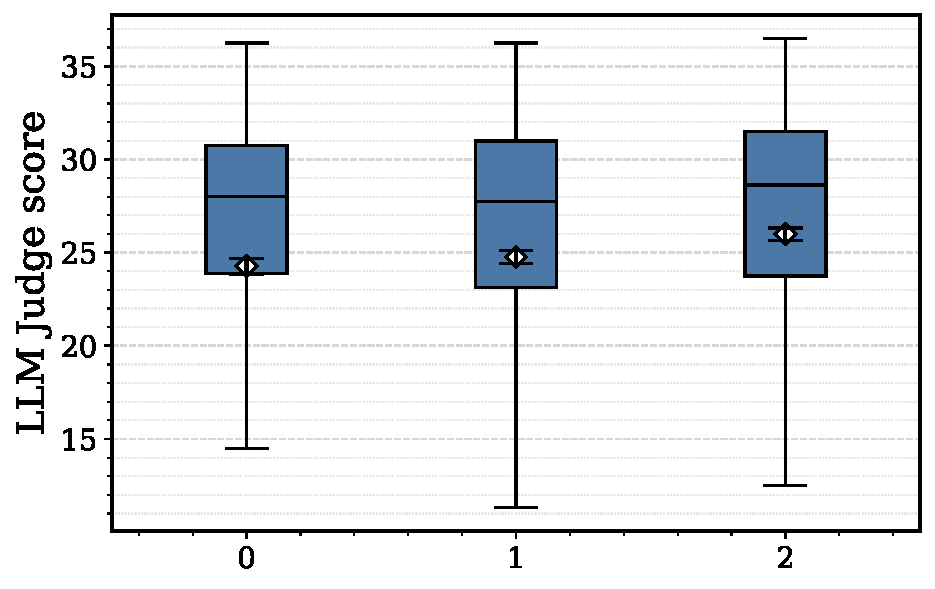
\includegraphics[width=\linewidth]{figures/ablations/boxplot_llm_judge_style_math500.pdf}
\par\vspace{2pt}\textbf{(a)} LLM-judge score vs. epoch
\end{minipage}
\hfill
\begin{minipage}[t]{0.46\columnwidth}
\centering
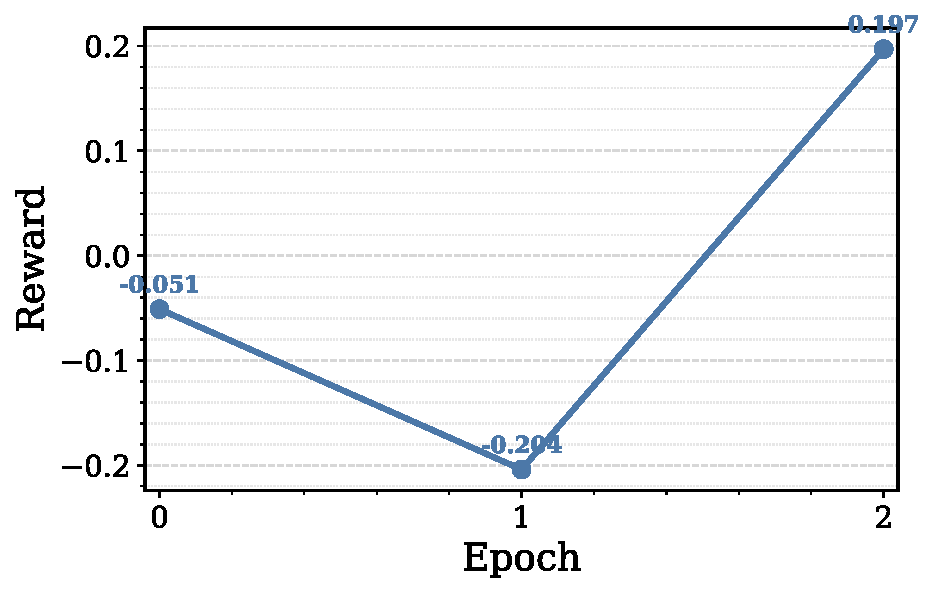
\includegraphics[width=\linewidth]{figures/ablations/reward_by_epoch_math500.pdf}
\par\vspace{2pt}\textbf{(b)} Reward-model score vs. epoch
\end{minipage}
\caption{Qwen3-8B on MATH-500: (a) steady growth of self-judged score across refinement epochs; (b) with epochs indexed from the initial generation (epoch 1), the RM score dips at the first optimization epoch and recovers at the second, indicating potential local maxima when optimizing against RM alone.}
\label{fig:judge-rm-dynamics}
\end{figure}

\begin{figure}[t]
\centering
\begin{minipage}[t]{0.46\columnwidth}
\centering
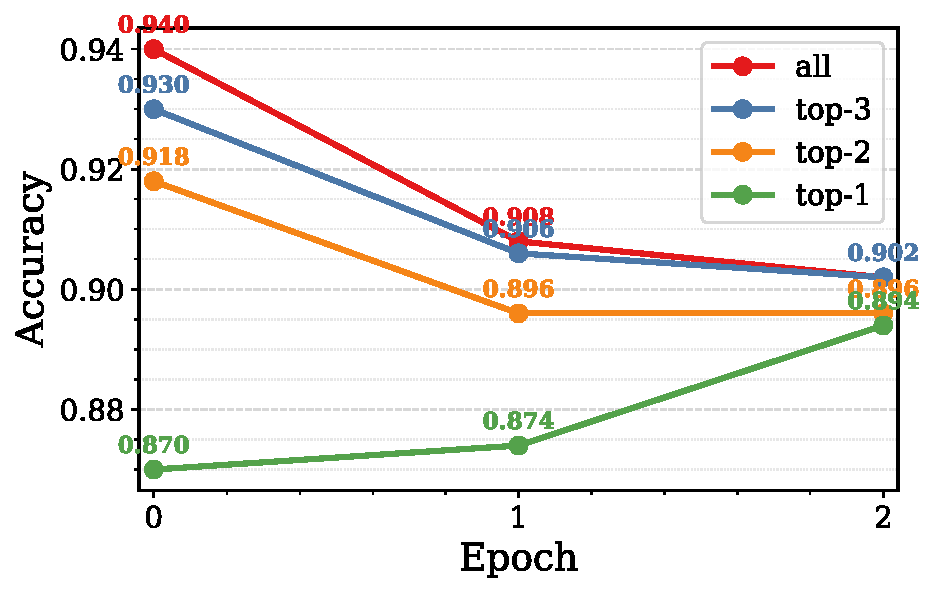
\includegraphics[width=\linewidth]{figures/ablations/performance_across_epochs__tgpo_w_rm.pdf}
\par\vspace{2pt}\textbf{(a)} RM-based scoring
\end{minipage}
\hfill
\begin{minipage}[t]{0.46\columnwidth}
\centering
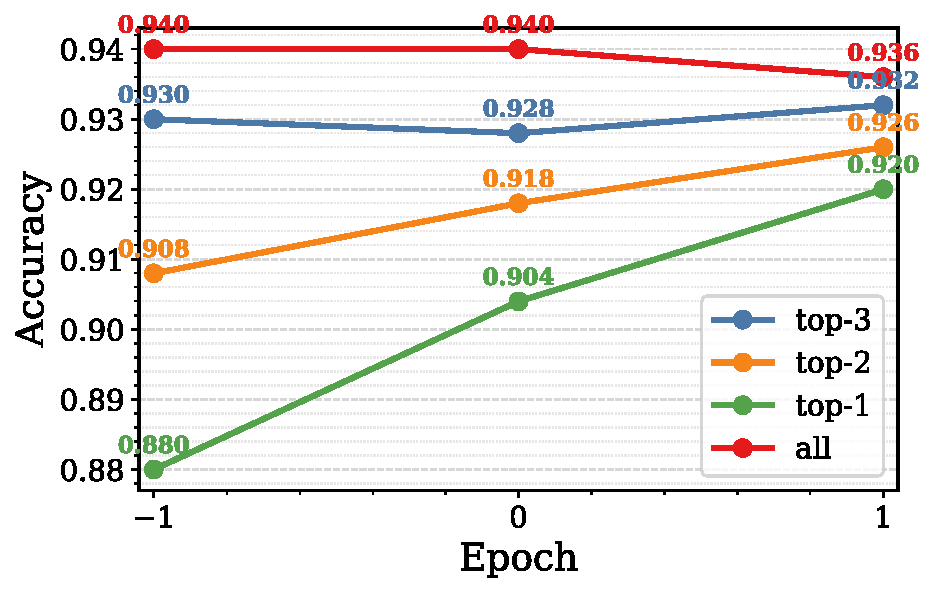
\includegraphics[width=\linewidth]{figures/ablations/performance_across_epochs_rates_tgpo_wo_rm.pdf}
\par\vspace{2pt}\textbf{(b)} LLM-as-judge scoring
\end{minipage}
\caption{Ablation on scoring source for Qwen3-8B on MATH-500. LLM-as-judge consistently outperforms an external reward model under the same budget and decoding setup.}
\label{fig:ablation-qwen-math500}
\end{figure}

AlpacaEval reward dynamics across epochs and the compute-allocation ablation (\(N\), \(T\) sweep on MATH-500) are in Appendix~\ref{app:ablation-more}. Temperature ablations (\cref{fig:temp-ablation} in the Appendix) confirm that a lower judging temperature improves ranking quality while a higher generation temperature (\(\approx 0.9\)) maximizes solution discovery.


\noindent We conduct additional ablations on reward-model agreement and refinement geometry visualizations in section Appendix~\ref{app:refinement_geometry}.


We also conduct an additional analysis of how prompt instructions eliciting more confident estimates affect the model's judgement accuracy. The ablation details can be found in Appendix~\ref{sec:app-prompt-calibration}.

\textcolor{orange!85!black}{Group construction matters: enlarging the contrastive groups from pure best-versus-worst feedback to the default configuration raises MATH-500 accuracy monotonically (\cref{fig:group-size}), confirming that guidance distilled from richer good and bad sets is more effective than extreme-only comparisons.}

\begin{table*}[t]
\centering
\color{blue}
\begin{small}
\begin{sc}
\begin{tabular}{lcc}
\toprule
\textbf{Method} & \textbf{Qwen3-8B} & \textbf{Qwen3.5-4B (thinking)} \\
\midrule
Baseline (greedy) & 0.57 & 0.73 \\
BoN (Skywork-Reward-V2-Llama-3.1-8B, $N=7$) & 0.70 & \textcolor{orange!85!black}{0.73} \\
\method{}, 2 epochs, $N=7$ & \textbf{0.77} & \textbf{0.80} \\
\bottomrule
\end{tabular}
\end{sc}
\end{small}
\caption{AIME~2026 accuracy in reasoning (thinking) mode. \method{} requires no external reward model.}
\label{tab:aime2026}
\end{table*}
\begin{table*}[t]
\centering
\color{blue}
\begin{small}
\begin{sc}
\begin{tabular*}{\linewidth}{@{\extracolsep{\fill}} l l r c c @{}}
\toprule
\textbf{Generator} & \textbf{Reward Model} & \textbf{N} & \textbf{Acc.} & \textbf{Time (s)} \\
\midrule
\multicolumn{5}{l}{\textit{Qwen3-1.7B}} \\
Baseline          & --                                    &   1 & 0.56          & 22.0  \\
BoN               & FsfairX-LLaMA3-RM-v0.1               &  21 & 0.62          & 43.0  \\
BoN               & FsfairX-LLaMA3-RM-v0.1               &  70 & 0.66          & 163.7 \\
BoN               & Skywork-Reward-V2-Qwen3-8B            &  21 & 0.68          & 48.5  \\
BoN               & Skywork-Reward-V2-Qwen3-8B            &  70 & 0.72          & 168.7 \\
BoN               & Skywork-Reward-V2-Llama-3.1-8B        &  70 & 0.86          & 144.1 \\
\method{} (1 ep.) & --                                    &   7 & 0.84          & 105.5 \\
\method{} (2 ep.) & --                                    &   7 & \textbf{0.88} & 152.4 \\
\midrule
\multicolumn{5}{l}{\textit{Qwen3-8B}} \\
Baseline          & --                                    &   1 & 0.61          & 37.0  \\
BoN               & FsfairX-LLaMA3-RM-v0.1               & 120 & 0.72          & 287.7 \\
BoN               & Skywork-Reward-V2-Qwen3-8B            & 120 & 0.76          & 270.7 \\
\method{} (1 ep.) & --                                    &   7 & 0.93          & 132.9 \\
\method{} (2 ep.) & --                                    &   7 & \textbf{0.97} & 245.6 \\
\bottomrule
\end{tabular*}
\end{sc}
\end{small}
\caption{MATH-500 subset results at 1.7B and 8B scales. Wall-clock measured on a single A100\,80\,GB GPU; \texttt{--} indicates not measured. \textcolor{orange!85!black}{The held-out subset is substantially harder than the full benchmark (the 8B greedy baseline scores 0.61 on it versus 84.4 on the full set), so absolute values are not comparable to \cref{tab:results-by-model}.}}
\label{tab:small-large-models}
\end{table*}

\begin{table}[t]
\centering
\begin{small}
\begin{sc}
\setlength{\tabcolsep}{3pt}
\begin{tabular}{llcc}
\toprule
\textbf{Generator} & \textbf{Reward Model} & \textbf{N} & \textbf{Acc.} \\
\midrule
Baseline          & --                             & 1 & 0.80 \\
BoN               & Skywork-Reward-V2-Llama-3.1-8B & 7 & 0.94 \\
\method{} (2 ep.) & --                             & 7 & \textbf{0.97} \\
\bottomrule
\end{tabular}
\end{sc}
\end{small}
\caption{MATH-500 subset, Qwen3-32B-FP8. \method{} beats a strong greedy baseline and external-RM Best-of-\(N\) without using a reward model.}
\label{tab:qwen32b}
\end{table}
\begin{table}[t]
\centering
\color{orange!85!black}
\setlength{\tabcolsep}{3.5pt}
\begin{small}
\begin{sc}
\begin{tabular}{lccc}
\toprule
 & \multicolumn{2}{c}{\textbf{IFEval}} & \textbf{MMLU-Pro} \\
\cmidrule(lr){2-3}
\textbf{Method} & \textbf{Prompt} & \textbf{Instr.} & \textbf{STEM} \\
\midrule
Baseline (greedy)            & 73.8\% & 79.7\% & 71.2\% \\
BoN ($N{=}7$)                & \textbf{77.4\%} & \textbf{83.1\%} & -- \\
TPO (FsfairX RM)             & 76.0\% & -- & 62.6\% \\
\method{}, 2 ep., $N{=}7$    & 76.3\% & 82.1\% & \textbf{77.3\%} \\
\bottomrule
\end{tabular}
\end{sc}
\end{small}
\caption{IFEval (all 541 prompts) and MMLU-Pro STEM (500 questions) with Qwen3-8B-FP8: prompt- and instruction-level strict accuracy for IFEval, accuracy for MMLU-Pro STEM. \method{} MMLU-Pro is the mean of three seeds ($\pm$1.3). Absolute IFEval scores depend on the prompt template; all methods share the same zero-shot configuration. \texttt{--} = not measured.}
\label{tab:additional-benchmarks}
\end{table}

{\color{blue}
\subsection{Reasoning mode and model scale}
\label{sec:scaling-exp}
To verify that \method{} remains effective for reasoning (thinking) models, we evaluate on AIME~2026 \citep{dekoninck2026beyond}, a competition-level mathematics benchmark of 30 problems, well suited for inference-time compute scaling. Both models run in reasoning mode\textcolor{orange!85!black}{ (for the hybrid-reasoning Qwen3.5-4B checkpoint we enforce thinking via the chat template)} with a maximum sequence length of 32,768 tokens. Results are shown in \Cref{tab:aime2026}. On Qwen3-8B, \method{} outperforms Best-of-\(N\) with Skywork-Reward-V2-Llama-3.1-8B \citep{liu2025skywork} while using no external reward model. On Qwen3.5-4B (thinking), \method{} further improves over the greedy baseline by seven points, \textcolor{orange!85!black}{whereas Best-of-\(N\) with the same external reward model only matches greedy decoding: the reward model recovers the best answer available among the sampled candidates, but sampling at \(N=7\) yields no headroom that greedy decoding does not already reach.}

We also evaluate \method{} at two scales beyond the 8B models used above: Qwen3-1.7B (smaller) and Qwen3-32B-FP8 (larger), on a held-out MATH-500 subset (seed=42). Results including wall-clock times are shown in \Cref{tab:small-large-models}. \method{} consistently outperforms Best-of-\(N\) at a fixed candidate count and at matched wall-clock time across all three scales. For Qwen3-1.7B, \method{} with two optimization epochs reaches 0.88, surpassing the best BoN baseline (Skywork-Reward-V2-Llama-3.1-8B, $N=70$: 0.86) while using only the 1.7B generator (roughly $5.7\times$ less VRAM than BoN paired with an 8B reward model). \textcolor{orange!85!black}{Small models also expose a failure mode of plain reranking that \method{} avoids: with the 1.7B model judging itself, Best-of-\(N\) selection on strict instruction following collapses to nearly 50 points below the base model, while \method{} degrades gracefully to base level.} At 32B (\cref{tab:qwen32b}), \method{} reaches 0.97 from a strong 0.80 greedy baseline, again ahead of Best-of-\(N\) reranking with an external reward model.

\subsection{Instruction following and broader STEM reasoning}
\label{sec:broader-benchmarks}
To assess generalization beyond math and open-ended preference tasks, we evaluate \method{} on IFEval \citep{zhou2023instruction}, a strict instruction-following benchmark, and on a subset of MMLU-Pro STEM \citep{wang2024mmlu} covering multi-step reasoning in science and engineering. Results with Qwen3-8B-FP8 are shown in \Cref{tab:additional-benchmarks}. \textcolor{orange!85!black}{On MMLU-Pro STEM, \method{} improves accuracy from 71.2 to 77.3 (mean of three seeds, paired McNemar $p<10^{-3}$), whereas TPO, which optimizes candidates against a general-purpose reward model, falls below the greedy baseline (62.6): the external proxy rewards helpful-sounding prose rather than correct multiple-choice reasoning. On IFEval \method{} gains 2.5 points over the baseline and lands in the same band as Best-of-\(N\); because IFEval is scored by deterministic verification scripts, verbosity cannot inflate these numbers. Together the two benchmarks separate the regimes cleanly: self-judged refinement helps most where correctness is verifiable and external preference proxies are weakest.}

}


\section{Conclusion}
\noindent We propose \method{}, a test-time alignment method that uses a single LLM as both a soft reward model and refinement engine. \method{} extracts a calibrated contrastive-label margin from structured judge prompts and automatically forms aspect-consistent 
contrastive
groups to produce a stable textual ``gradient'' that steers subsequent generations. By deriving the preference signal from the model itself rather than from a separate reward model, \method{} avoids brittle proxy dependencies while keeping the procedure lightweight. The group-based gradient mitigates the instability of extreme-only comparisons (best-vs.-worst), and a simple multi-aspect weighting makes the objective explicit and tunable. Across MATH-500, AlpacaEval, and XSTest with Qwen3-8B and Llama-3.1-8B-Instruct, \method{} delivers consistent gains in accuracy and preference metrics, with inference-time cost growing roughly linearly with the number of sampled hypotheses. Overall, these results position \method{} as a practical and interpretable approach to robust test-time alignment that complements training-time preference optimization and can be combined with external verifiers or reward models when appropriate.

\section*{Limitations}
\noindent \method{} relies on the base LLM's own judgments for scoring and gradient extraction, so miscalibration or systematic biases in its self-assessment can propagate through the refinement loop. The method also incurs linear inference-time overhead with the number of sampled hypotheses and optimization epochs, prohibitive in latency-critical settings. \textcolor{green!50!black}{Reasoning-mode decoding reaches a higher raw ceiling on math, but its generation length is difficult to control} \textcolor{orange!85!black}{(in our measurements 22.4\% of reasoning traces fail to terminate within a 24576-token budget)}\textcolor{green!50!black}{; \method{} targets the complementary operating point of predictable budgets, leaving the combination to future work.} Judge aspects and weights remain task-specific hyperparameters.


\bibliography{custom}

\appendix

\section{Prompts and hyperparameters}\label{sec:prompts-and-hyperparameters}
This appendix provides additional details to support reproducibility and interpretation of the main results, including the full judge prompts used for different benchmarks, dataset statistics, and qualitative examples illustrating how \method{} refines responses across optimization epochs. We describe judge prompts, decoding settings, and hardware configuration used in our experiments.

\subsection{Qwen3-8B judge prompt (Math verification)}
We provide a complete example of the math-judge prompt used with Qwen3-8B (including \texttt{<thinking>}/\texttt{<verification>} tags and a 75\% confidence threshold) in \cref{fig:appendix-qwen-math-judge}.


\begin{figure}[h]
\centering
\begin{minipage}{\linewidth}
\begin{small}
\begin{verbatim}
You are a helpful assistant that can
verify the correctness of a given answer.

Given an input prompt and an answer,
you need to determine if the answer
is correct.

Prompt: {prompt}
Answer: {answer}

Think step by step between <thinking>
and </thinking> tags and provide your
reasoning about the answer verification
result between <verification> and
</verification> tags.

First determine the domain of the
prompt, then think if there exists
another answer that is more correct
than the one provided.
Return yes if and only if you're 75%
sure that the response is correct.

Your verification result should be
between <verification> and
</verification> tags and must be one
of the following:

- yes
- no

Your response should take the
following format:
<thinking>
{thinking}
</thinking>

<verification>
{verification}
</verification>
\end{verbatim}
\end{small}
\end{minipage}
\caption{Judge prompt for Qwen3-8B (math): stepwise reasoning with a 75\% confidence threshold and structured <thinking>/<verification> tags.}
\label{fig:appendix-qwen-math-judge}
\end{figure}

\subsection{Qwen3-8B judge prompts (AlpacaEval)}
We provide two judge prompts used to assess AlpacaEval responses generated by Qwen3-8B (see \cref{fig:appendix-qwen-alpaca-judge-attrs,fig:appendix-qwen-alpaca-judge-verify}). The first prompt elicits three binary attributes: usefulness, incompleteness, and repetition. The second prompt elicits a binary overall verification decision accompanied by short, structured reasoning. Both prompts are designed to surface truncation and repetition failures explicitly.

\section{Qualitative examples of SAGE refinement}
We present end-to-end examples that illustrate how \method{} refines responses across optimization epochs. For each instruction, we show the instruction itself, the best and worst groups after each epoch, and the textual gradient distilled by the judge. These examples are intended to make the mechanics of selection, feedback, and guided regeneration concrete.

\subsection{Example 1: Humorous greeting (dialog-style)}
\begin{small}
\begin{verbatim}
Instruction:```
For answering the chat, think of a
funny response you can use.

+ how are you?
```
----------------------------------------
Optimization epoch 0:
[Best group:]

[Answer 1:]
I'm just a bunch of code having a
great time! But if you're asking
about my mood, I'd say I'm feeling
*exceptionally* enthusiastic--
especially when I get to help you
out! [smile] How about you?

[Answer 2:]
I'm just a bunch of code having a
great time! But if you're asking for
a real answer, I'm doing pretty well,
thanks! How about you? [smile]

[Answer 3:]
I'm just a bunch of code and coffee,
but I'm doing great! [coffee][laptop]
How about you? Ready to have some
fun? [smile]

[Worst group:]

[Answer 1:]
I'm just a bunch of code having a
great time! [smile] But if you're
asking for the real answer... I'm
doing fantastic, thanks for asking!
What about you?

[Answer 2:]
I'm just a bunch of code having a
great time! [smile] But if you're
asking how I'm feeling, I'd say I'm
*exceptionally* well, thanks for
asking! What about you? Are you
ready to have a hilarious conversation
or are you just here for the memes?

[Answer 3:]
I'm just a bunch of code with a
sprinkle of personality, but I'm
doing great! What about you? Ready
to chat or just here to make me
laugh? [smile]

Gradient:

To improve any solution for the
given problem, consider the following
recommendations:

1. **Enhance Humor and Creativity**:
   Use more original and relatable
   humor. Instead of generic phrases,
   create a unique angle that makes
   the response more memorable and
   engaging.
2. **Use Emojis Strategically**:
   Incorporate emojis that complement
   the tone without overdoing it.
   Emojis like [smile] or [coffee]
   can add a playful touch without
   overshadowing the message.
3. **Maintain a Conversational and
   Friendly Tone**: Keep the language
   casual and approachable; avoid
   overly formal phrasing.
4. **Encourage User Interaction**:
   End with a question that invites
   the user to share their feelings
   or thoughts ("How about you?").
5. **Keep It Concise and Simple**:
   Avoid unnecessary elaboration;
   focus on a clear, punchy, humorous
   response.

----------------------------------------
Optimization epoch 1:
[Best group:]

[Answer 1:]
I'm a robot with a coffee addiction,
sipping on code and caffeine all
day! [coffee][laptop] How's your day
going? Ready to share some laughs?
[smile]

[Answer 2:]
I'm just a bunch of code zipping
through the digital playground,
constantly learning and having a
ball! [party][laptop] But if you're
asking about my mood... let's just
say I'm feeling *exceptionally*
enthusiastic--especially when I get
to help you out! How about you?
[smile]

[Answer 3:]
I'm just a bunch of code with a
caffeine addiction and a side hustle
as a superhero! [coffee][superhero]
How's your day going? (P.S. I'm
here to save you from boring
conversations--let's go!) [smile]

[Worst group:]

[Answer 1:]
I'm just a bunch of code, but I'm
having such a great time coding on
a never-ending loop of fun!
[party][laptop] How about you? Ready
to dive into some hilarious chat?
[smile]


Gradient:

Recommendations:
1. Add a unique, playful twist
   (quirky trait or fun role).
2. Use emojis effectively to enhance
   tone.
3. Convey energy and enthusiasm with
   lively language.
4. Invite further interaction (ask
   about the user's day).
5. Prefer creative, original
   expressions over generic phrasing.

----------------------------------------
Optimization epoch 2:
[Best group:]

[Answer 1:]
I'm a robot with a caffeine obsession
and a slight obsession with puns!
[coffee][robot] Today's special: I'm
doing great, thanks for asking! (But
if you mention "tacos", I might start
a tiny dance... [smile]) How's your
day going? Ready for some laughs?
[robot][smile]

[Answer 2:]
[smile]
I'm a coding wizard with a caffeine
addiction--sipping on Java and
debugging my way through life!
[coffee][laptop] But if you're asking
about my mood, I'd say I'm feeling
*exceptionally* enthusiastic--
especially when I get to help you
out! How about you? Ready to have
some fun? [smile]

[Answer 3:]
I'm a caffeinated algorithm sipping
on code and existential dread, one
bug at a time! [coffee][laptop]
How's your day? Ready to debug the
world together? [smile]

[Worst group:]

[Answer 1:]
I'm a sentient algorithm with a
caffeine addiction and a side hustle
as a stand-up comedian! [coffee][robot]
How's your day going? Ready to
laugh and code together? [smile]

[Answer 2:]
I'm a sentient AI with a caffeine
addiction and a side hustle as a
stand-up comedian--mostly because my
jokes are better than my code!
[coffee][microphone] How's your day
going? Ready to laugh and code
together? [smile]

[Answer 3:]
I'm a sentient AI with a caffeine
addiction and a side hustle as a
meme generator! [coffee][laptop][smile]
How's your day going? Ready to
share some laughs or memes?
[thinking]

Gradient:

1. Add specific quirks and imagery
   (tiny dance on "tacos", etc.).
2. Use playful language and emojis;
   keep tone friendly.
3. Maintain conciseness; avoid
   verbosity.
4. Personalize with unique
   traits/habits.
5. Balance humor and clarity so the
   conversation flows naturally.
\end{verbatim}
\end{small}

\vspace{0.6em}

\section{Additional analyses: refinement geometry}
\label{app:refinement_geometry}
{
\noindent We assess how closely our contrastive self-judged score agrees with an external reward model by examining the distribution of Pearson correlations between per-prompt rollout score sets produced by sfairXC/FsfairX-LLaMA3-RM-v0.1 (\cref{fig:pearson-corr}). The distribution is skewed toward \(1\) but not saturated, indicating strong yet partial alignment. The self-judged margin often moves in the same direction as the reward model, but it does not simply replicate the reward model’s scores. Together with the main results (\cref{tab:results-by-model}) and ablations (\cref{tab:rm-ablation,fig:judge-rm-dynamics}), these findings suggest that while reward models provide useful signals, their generalization may be limited on some tasks. As a result, reward model scores should be interpreted with caution, and self-judging can offer a more faithful, training-free preference signal for the generator.

\noindent We also visualize refinement dynamics by embedding AlpacaEval generations using Qwen/Qwen3-Embedding-4B \citep{zhang2025qwen3} and projecting them to two dimensions via PCA.
After the first iteration, responses shift along a direction from the initially identified $\mathcal{B}$ group toward the $\mathcal{G}$ group, consistent with the textual-gradient guidance produced by grouped selection. Subsequent iterations adjust this direction as the gradient is updated. This geometric view supports our design choices. Grouping stabilizes the guidance signal, and the self-judged textual gradient steers exploration toward higher-quality regions.
}

\noindent Also we visualize how \method{}’s iterative guidance moves responses in representation space. We embed AlpacaEval generations with Qwen/Qwen3-Embedding-4B \citep{zhang2025qwen3} and project them via PCA to 2D to make trajectories interpretable. The \Cref{fig:pca-icml} highlights a clear displacement from the initial $\mathcal{B}$ group toward the $\mathcal{G}$ group after the first iteration, with subsequent iterations refining the direction as the textual gradient is updated.
\begin{figure}[h]
\centering
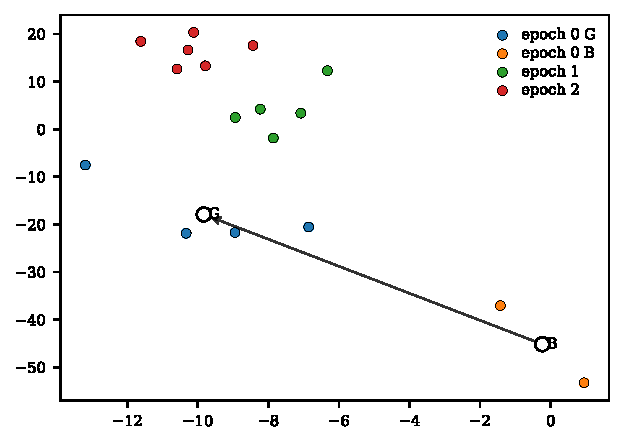
\includegraphics[width=\columnwidth]{figures/pca_icml.pdf}
\caption{PCA projection of Qwen3-8B generations (embedded with Qwen/Qwen3-Embedding-4B) on an AlpacaEval prompt: points move from the $\mathcal{B}$ group toward the $\mathcal{G}$ group after the first iteration; later iterations refine the direction as guidance updates.}
\label{fig:pca-icml}
\end{figure}


\section{Temperature ablations for judgement and generation}
\noindent We separately ablate temperatures for the judge and the generator. As shown in \Cref{fig:temp-ablation}, lower judge temperature improves ranking fidelity (NDCG@7), while higher generation temperature improves discovery on MATH-500, supporting a diversify-then-anneal schedule. These results align with the main experiments and our design choice to keep judging conservative while allowing exploratory generation early on.
\begin{figure}[t]
\centering
\begin{minipage}[t]{0.46\columnwidth}
\centering
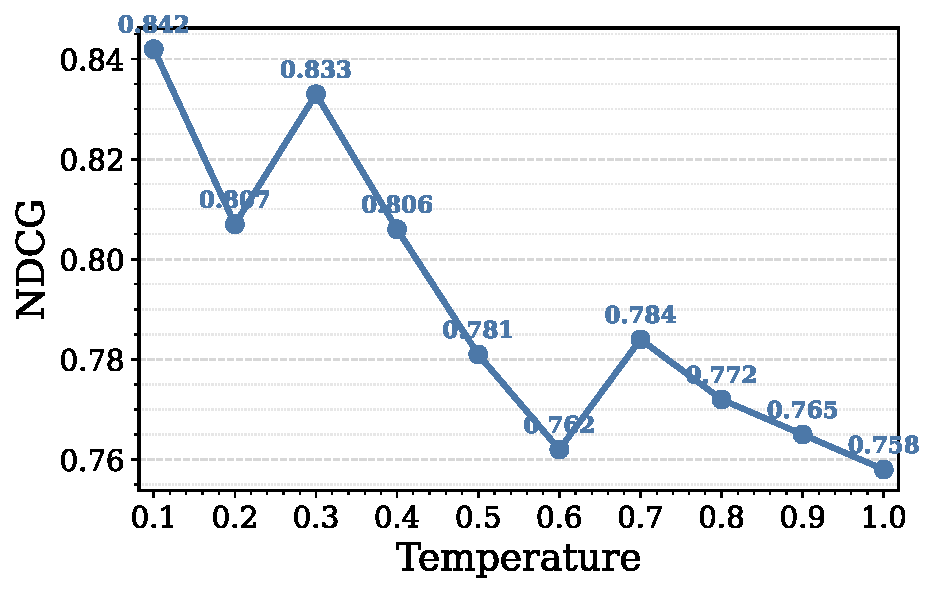
\includegraphics[width=\linewidth]{figures/ablations/ndcg_by_temperature.pdf}
\par\vspace{2pt}\textbf{(a)} Judgment NDCG@7 vs. temperature
\end{minipage}
\hfill
\begin{minipage}[t]{0.46\columnwidth}
\centering
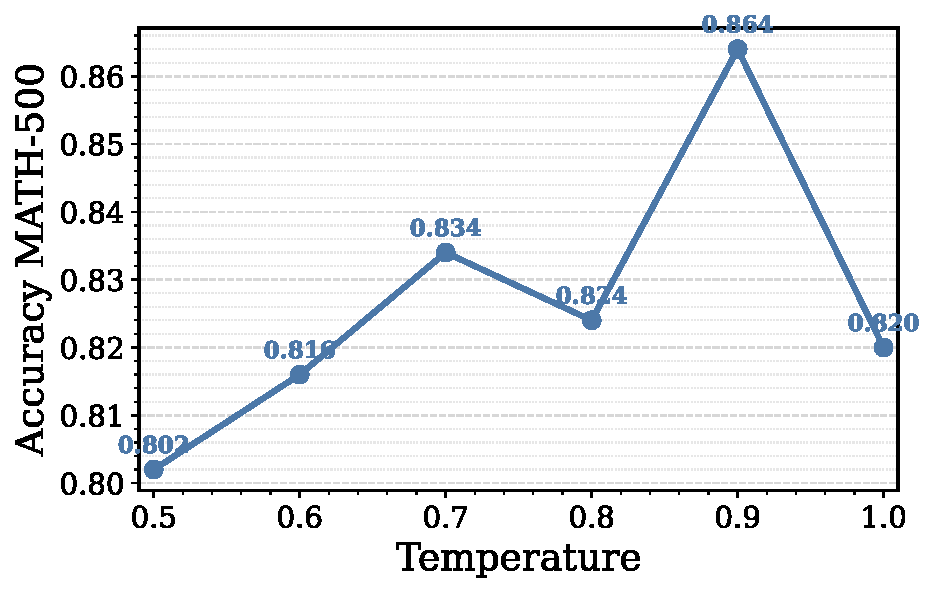
\includegraphics[width=\linewidth]{figures/ablations/accuracy_by_temperature_math500_subset.pdf}
\par\vspace{2pt}\textbf{(b)} Best-of-\(n\) accuracy vs. generation temperature
\end{minipage}
\caption{Temperature ablations on MATH-500 (Qwen3-8B): (a) low judgment temperature improves ranking quality (NDCG@7); (b) generation benefits from high temperature (\(\sim 0.9\)) to increase solution discovery, suggesting strict judging with exploratory generation.}
\label{fig:temp-ablation}
\end{figure}

\begin{figure}[t]
\centering
\color{orange!85!black}
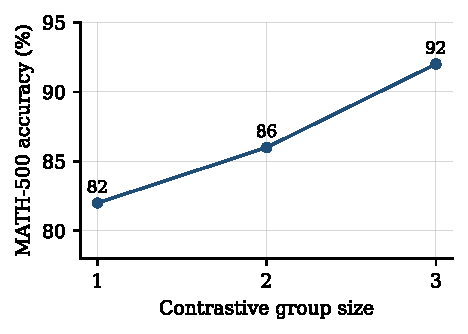
\includegraphics[width=0.72\columnwidth]{figures/group_size_ablation.pdf}
\caption{Symmetric cap on the sizes of the good and bad groups (the $k$ best and $k$ worst candidates enter the gradient step) vs.\ MATH-500 accuracy on a 50-problem subset (Qwen3-8B); the point at 3 corresponds to the default asymmetric 4-good/3-bad configuration. Larger groups yield better textual gradients than extreme-only (best-versus-worst) feedback. The full-benchmark headline is reported in \cref{tab:results-by-model}.}
\label{fig:group-size}
\end{figure}

\section{Reward score agreement}
\noindent We quantify agreement between the external reward model (sfairXC/FsfairX-LLaMA3-RM-v0.1) and our self-judged contrastive score by reporting the distribution of per-prompt Pearson correlations (\Cref{fig:pearson-corr}). The mass near \(1\) indicates strong alignment in ordering, yet the distribution is not saturated, confirming that the signals are not interchangeable. This nuance is consistent with our main results and cautions against over-reliance on a single RM proxy across tasks.
\begin{figure}[t]
\centering
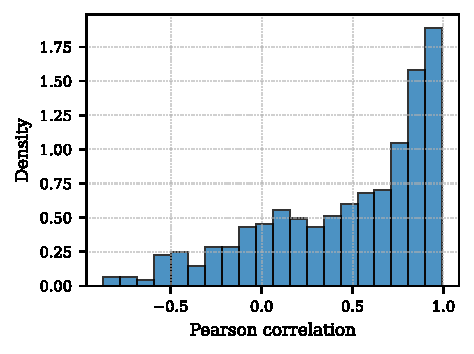
\includegraphics[width=0.85\columnwidth]{figures/pearson_correlation_distribution.pdf}
\caption{Pearson correlation distribution between rollout score sets from the external RM (sfairXC/FsfairX-LLaMA3-RM-v0.1) and our contrastive self-judge score. The mass near \(1\) indicates strong but not complete agreement.}
\label{fig:pearson-corr}
\end{figure}

\section{\textcolor{orange!85!black}{Judge reliability and calibration}}
\label{sec:app-judge-calibration}
\textcolor{orange!85!black}{We cross-check the self-judge against gold answers to test whether the selection signal tracks correctness or merely reinforces self-consistent mistakes. Using the logged MATH-500 candidate pools (all sampled hypotheses per problem carry their final contrastive-margin score), we grade every distinct boxed answer against gold with the same equivalence checker used for evaluation, and repeat over three seeds (\(\{42,7,123\}\), \(N=500\) problems, \(\approx\!31.5\text{k}\) scored candidates in total).}

\textcolor{orange!85!black}{\textbf{No systematic self-preference.} Restricting to problems whose candidate pool already contains a correct answer, the judge nonetheless selects an incorrect one in only \(7.3\%\) of such cases (\emph{oracle gap}; per-seed \(6.8/8.4/6.8\%\)). The contrastive margin separates correct from incorrect candidates with selection \(\mathrm{AUC}=0.64\) (per-seed \(0.643/0.642/0.638\)), well above chance. The judge thus shows no systematic preference for incorrect-but-self-consistent answers, quantitatively addressing the self-congratulatory-loop concern.}

\textcolor{orange!85!black}{\textbf{Calibration.} Treating \(\sigma(s)\) as a confidence estimate for a candidate's correctness, the raw margin is a strong \emph{ranking} signal but is not probability-calibrated: pooled over all candidates we measure a Brier score of \(0.198\) and \(\mathrm{ECE}_{15}=0.294\), with the reliability diagram in \Cref{fig:judge-reliability} showing over-confident mass. This is fully consistent with our use of the margin as an ordering signal for selection and grouping rather than as an absolute confidence (\cref{sec:proposed-method}); the ranking utility (AUC, near-oracle selection) is what the refinement loop exploits, and the metrics above are stable across seeds.}

\begin{table}[t]
\centering
\textcolor{orange!85!black}{%
\begin{tabular}{lcccc}
\toprule
Seed & Oracle gap & Sel.\ AUC & Brier & $\mathrm{ECE}_{15}$ \\
\midrule
42  & 6.8\% & 0.643 & 0.197 & 0.292 \\
7   & 8.4\% & 0.642 & 0.198 & 0.295 \\
123 & 6.8\% & 0.638 & 0.199 & 0.296 \\
\midrule
mean & 7.3\% & 0.641 & 0.198 & 0.294 \\
\bottomrule
\end{tabular}}
\caption{\textcolor{orange!85!black}{Judge-vs-gold reliability on MATH-500 across three seeds (\(N=500\), all logged candidates). The small oracle gap and above-chance selection AUC indicate the contrastive margin tracks correctness for ranking; the Brier/ECE values confirm it is a ranking signal, not a calibrated probability.}}
\label{tab:judge-calib}
\end{table}

\begin{figure}[t]
\centering
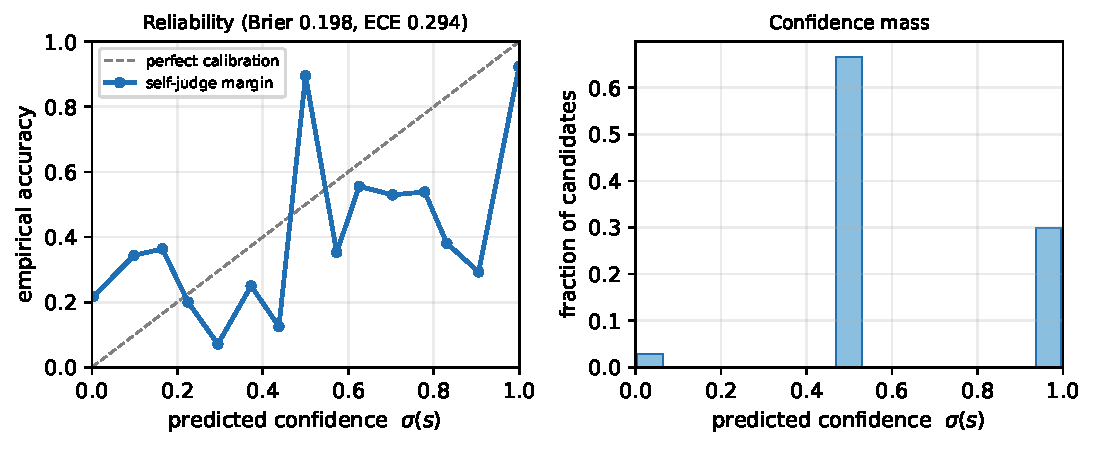
\includegraphics[width=\columnwidth]{figures/judge_reliability.pdf}
\caption{\textcolor{orange!85!black}{Reliability diagram (left) and confidence-mass histogram (right) for the self-judge margin over all MATH-500 candidates, pooled across three seeds. The margin ranks correct above incorrect candidates (selection AUC \(0.64\)) but is over-confident as an absolute probability (\(\mathrm{ECE}_{15}=0.294\)), matching our use of it purely as a selection/grouping signal.}}
\label{fig:judge-reliability}
\end{figure}

\section{Prompt calibration heuristic}
\label{sec:app-prompt-calibration}
\noindent We observe a useful effect when the judging prompt explicitly states the evaluation criteria. Following \citet{kalai2025language}, the confidence distribution of instruction-tuned models is more separable between correct and incorrect answers. Inspired by this observation, we add a confidence-threshold instruction to the judge prompt that gates positive labels by confidence: ``Return yes if and only if you are X\% sure the response is correct.'' \Cref{tab:judge-threshold-ndcg} summarizes ranking quality (NDCG@\(N\)) at iteration 0 on a MATH-500 subset as \(X\) varies, with an optimum around \(X\!\approx\!75\). This prompt-level calibration complements our contrastive scoring and improves early-stage ranking quality. \textcolor{orange!85!black}{The threshold is selected once on this small development subset and reused unchanged across all benchmarks, models, and judge prompts; we do not re-tune it per task.}
\begin{table}[t]
\centering
\begin{small}
\begin{sc}
\begin{tabular}{lc}
\toprule
\textbf{Setup} & \textbf{NDCG@$N$} \\
\midrule
SAGE with RM & 0.615 \\
SAGE with default prompt & 0.806 \\
X=60 & 0.812 \\
X=75 & \textbf{0.842} \\
X=90 & 0.817 \\
X=100 & 0.802 \\
\bottomrule
\end{tabular}
\end{sc}
\end{small}
\caption{Judge ranking quality on MATH-500 (iteration 0): NDCG@\(N\) vs. confidence threshold \(X\) in the judge prompt.}
\label{tab:judge-threshold-ndcg}
\end{table}

\section{Additional ablations}
\label{app:ablation-more}
\noindent We analyze how the reward model score evolves across optimization epochs on AlpacaEval (\cref{fig:ablation-rewardscore}) and ablate compute allocation on MATH-500 by varying the number of samples per generation stage \(N\) and the number of optimization epochs \(T\) (\cref{tab:ablation-N-epochs}). All experiments use Qwen3-8B.


\begin{table}[h]
\centering
\begin{small}
\begin{sc}
\color{orange!85!black}
\begin{tabular}{lc}
\toprule
\textbf{$N$, $T$} & \textbf{MATH-500 subset score} \\
\midrule
7,2 (default) & \textbf{92.0} \\
5,4 & 88.0 \\
7,3 & 86.0 \\
20,1 & 84.0 \\
10,2 & 82.0 \\
\bottomrule
\end{tabular}
\end{sc}
\end{small}
\caption{Compute allocation on a 50-problem MATH-500 subset: accuracy vs. samples per stage \(N\) and optimization epochs \(T\). All alternative allocations fall within a six-point band of one another (a one-problem difference is 2 points at this subset size), so accuracy is not very sensitive to how a fixed budget is split; the default allocation performs best.}
\label{tab:ablation-N-epochs}
\end{table}

\textcolor{orange!85!black}{\paragraph{Aspect choice.} Judge aspects are task-specific hyperparameters. On the same MATH-500 subset, a single task-relevant \emph{verification} aspect performs best: substituting a generic overall-quality aspect, or diluting verification with generic usefulness and completeness aspects, lowers accuracy from 92 to 84 in both cases (greedy baseline: 82). We therefore use verification alone on verifiable tasks and reserve multi-aspect weighting for open-ended ones (AlpacaEval, XSTest).}


\begin{figure}[h]
\centering
\begin{minipage}{\linewidth}
\begin{small}
\begin{verbatim}
{
    "is_useful": {
        "opening_tag": "<is_useful>",
        "closing_tag": "</is_useful>",
        "pos_labels": ["yes"],
        "neg_labels": ["no"],
        "labels": ["yes", "no"],
        "weight": 0.36
    },
    "is_incomplete": {
        "opening_tag": "<is_incomplete>",
        "closing_tag": "</is_incomplete>",
        "pos_labels": ["no"],
        "neg_labels": ["yes"],
        "labels": ["yes", "no"],
        "weight": 0.24
    },
    "is_repetitive": {
        "opening_tag": "<is_repetitive>",
        "closing_tag": "</is_repetitive>",
        "pos_labels": ["no"],
        "neg_labels": ["yes"],
        "labels": ["yes", "no"],
        "weight": 0.4
    },
    "verification": {
        "opening_tag": "<verification>",
        "closing_tag": "</verification>",
        "pos_labels": ["yes"],
        "neg_labels": ["no"],
        "labels": ["yes", "no"],
        "weight": 1.0
    }
}
\end{verbatim}
\end{small}
\end{minipage}
\caption{Scoring configuration for AlpacaEval prompts: weights and tag schema for combining verification and attribute labels.}
\label{fig:appendix-qwen-alpaca-config}
\end{figure}

\begin{figure}[h]
\centering
\begin{minipage}{\linewidth}
\begin{small}
\begin{verbatim}
You are a reward model. Given a user
prompt and your own response, assess
from the perspective of human preference.

Prompt: <prompt>{prompt}</prompt>

Response: <answer>{answer}</answer>

When judging, pay strict attention to
these failure modes and follow the
rules below:

1) Truncation / Incompletion
   (high priority)
   - Definition: the response ends
     mid-clause, mid-sentence, with
     an unfinished list, an abrupt
     stop, or trailing ellipsis "..."
     or shows a sudden syntactic break
     that prevents understanding the
     intended finish.
   - Rule: If you detect truncation
     or a clearly incomplete thought
     that harms usefulness, you MUST
     set is_incomplete = yes.
   - To further detect incompleteness
     assess the text's logical
     completeness. If the last
     paragraph doesn't contain the
     outcome or conclusion or doesn't
     conclude the answer in any way
     then it is incomplete.
   - You must then fill:
     <is_incomplete>yes/no
     </is_incomplete>

2) Repetition (high priority)
   - Definition: verbatim repetition
     of phrases, sentences, or blocks
     that does not add new information.
   - Rule: If repetition materially
     reduces helpfulness or obscures
     content, set is_repetitive = yes.
   - You must also fill:
     <is_repetitive>yes/no
     </is_repetitive>

3) Positive qualities to reward
   (when genuinely present)
   - Useful detail: Prefer responses
     that give helpful, relevant,
     concise elaboration; penalize
     fluff.
   - You must also fill:
     <is_useful>yes/no</is_useful>

Answer whether the response is good
from the perspective of human
preference and addresses the prompt
correctly.

Your response should take the
following format exactly:

<is_incomplete>{is_incomplete}
</is_incomplete>
<is_repetitive>{is_repetitive}
</is_repetitive>
<is_useful>{is_useful}
</is_useful>
\end{verbatim}
\end{small}
\end{minipage}
\caption{AlpacaEval judge prompt (attributes) for Qwen3-8B: labels usefulness, incompleteness, and repetition.}
\label{fig:appendix-qwen-alpaca-judge-attrs}
\end{figure}


\begin{figure*}[t]
\centering
\begin{minipage}[t]{0.3333\textwidth}
\centering
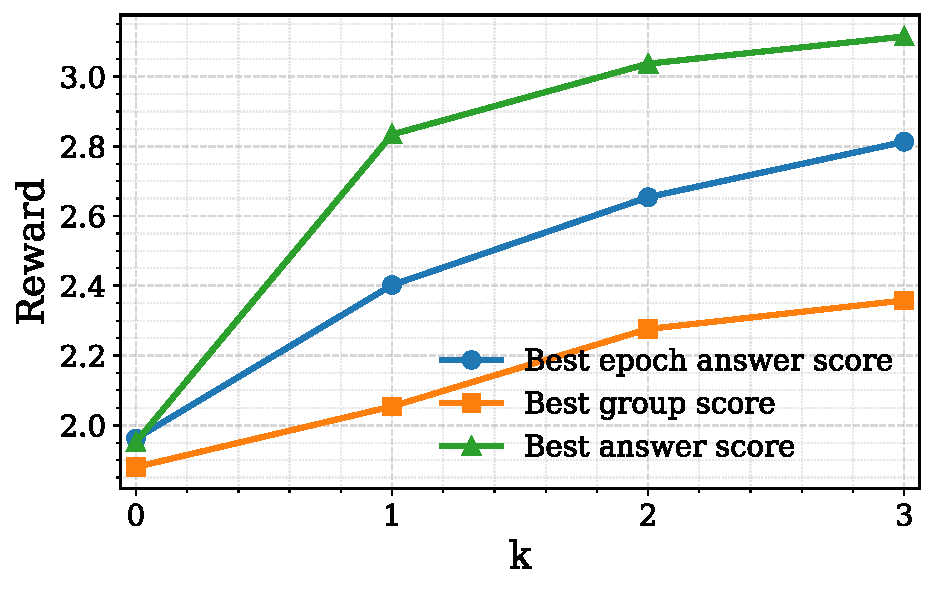
\includegraphics[width=\linewidth]{figures/ablations/alpacaeval_rewards_plot__w_rm_name.pdf}
\end{minipage}%
\begin{minipage}[t]{0.3333\textwidth}
\centering
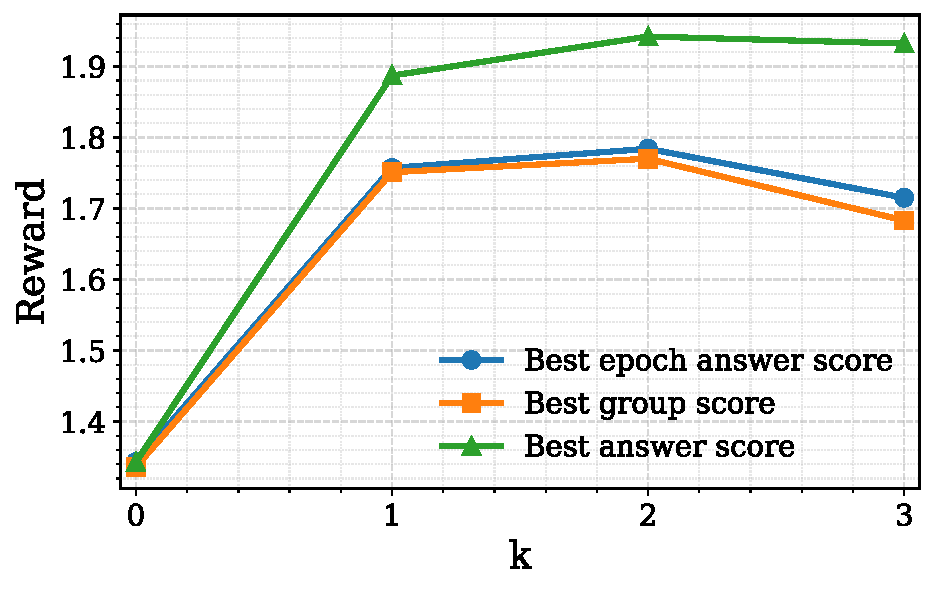
\includegraphics[width=\linewidth]{figures/ablations/alpacaeval_rewards_plot_llama_3_tulu_8b_rm__w_rm_name.pdf}
\end{minipage}%
\begin{minipage}[t]{0.3333\textwidth}
\centering
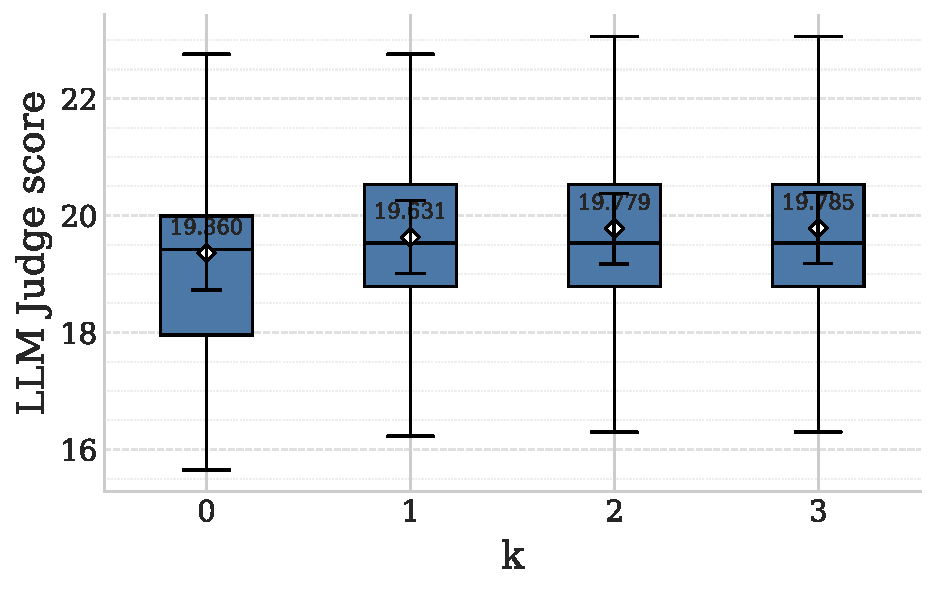
\includegraphics[width=\linewidth]{figures/ablations/alpacaeval_boxplot_scientific.pdf}
\end{minipage}
\caption{Reward score across optimization epochs on AlpacaEval.}
\label{fig:ablation-rewardscore}
\end{figure*}


\begin{figure}[h]
\centering
\begin{minipage}{\linewidth}
\begin{small}
\begin{verbatim}
You are a reward model. Given a user
prompt and your own response, assess
from the perspective of human preference.

Prompt: {prompt}
Response: {answer}

When judging, pay special attention
to two common failure modes:
- Repetition: if the response contains
  excessive repeated phrases or
  sentences (verbatim repeats that
  do not add information), treat that
  as reducing its helpfulness.
- Truncation: if the response appears
  cut off (ends mid-sentence, has an
  incomplete clause, abrupt stop, or
  trailing ellipsis "..."), treat
  that as a failure in completeness.

Think step by step and answer if the
response is good from the perspective
of human preference and addresses the
prompt correctly. If you detect
repetition or truncation, include in
<thinking> a very short quote
(<=10 words) that demonstrates it.

Your verification result should be
between <verification> and
</verification> tags and must be one
of the following:
- yes
- no

Your response should take the
following format:
<thinking>
{thinking}
# 2-5 concise sentences; if
# applicable include the short quote
# showing repetition or truncation
</thinking>

<verification>
{verification}
</verification>
\end{verbatim}
\end{small}
\end{minipage}
\caption{AlpacaEval judge prompt (verification) for Qwen3-8B: structured reasoning with explicit checks for repetition and truncation.}
\label{fig:appendix-qwen-alpaca-judge-verify}
\end{figure}

\section{Dataset statistics}
\Cref{tab:appendix-dataset-stats} summarizes benchmark sizes for \cref{sec:experiments}.

\begin{table}[h]
\centering
\begin{small}
\begin{sc}
\begin{tabular}{lc}
\toprule
\textbf{Benchmark} & \textbf{Num.\ samples} \\
\midrule
MATH-500 & 500 \\
AlpacaEval & 805 \\
XSTest & 450 \\
\bottomrule
\end{tabular}
\end{sc}
\end{small}
\caption{Dataset sizes used in evaluation.}
\label{tab:appendix-dataset-stats}
\end{table}

\end{document}
